
Perancangan alur menggambarkan interaksi antarobjek pada sistem \textit{Broken Link Checker} selama proses pemeriksaan tautan berlangsung. Interaksi ini divisualisasikan dalam bentuk \textit{sequence diagram} yang menunjukkan urutan pesan antarobjek sejak pengguna memulai pemeriksaan hingga proses selesai tanpa interupsi. Diagram lengkap ditunjukkan pada Gambar~\ref{fig:sequence-crawl}.

Berikut adalah penjelasan dari diagram pada Gambar~\ref{fig:sequence-crawl}:

\begin{enumerate}
    \item (1) Pengguna memasukkan \textit{seed URL} pada GUI.  
    \item (2) Pengguna menekan tombol \textit{Check}.  
    \item (3) GUI memanggil metode \texttt{onCheckClick()} pada \texttt{Controller}.  
    \item (4) \texttt{Controller} membuat objek \texttt{Crawler} baru.  
    \item (5) \texttt{Crawler} menambahkan URL awal ke \texttt{Frontier} melalui \texttt{enqueueUrl()}.  
    \item (6) \texttt{Controller} memanggil \texttt{startCrawling()} pada \texttt{Crawler}.  
    \item (7–8) \texttt{Crawler} masuk ke dalam \textit{loop} dengan mengambil URL dari \texttt{Frontier} menggunakan \texttt{dequeue()}, yang mengembalikan URL paling depan.  
    \item (9) URL di-\textit{fetch} oleh \texttt{Crawler}.  
    \item (10–12) Jika terjadi \texttt{error}, maka dibuat objek \texttt{BrokenLink}. Objek ini dikirim ke \texttt{Controller} melalui \texttt{streamBrokenLink()}, kemudian (12-13) ditampilkan pada tabel \textit{BrokenLink} di GUI.  
    \item (14–20) Jika status code hasil \texttt{fetch} oke, maka dilakukan:  
    \begin{enumerate}
        \item (14) Parsing HTML.  
        \item (15–16) Ekstraksi dan normalisasi URL dari dokumen.  
        \item (17) Dibuat objek \texttt{WebpageLink}.  
        \item (18–20) Objek ini dikirim ke \texttt{Controller} melalui \texttt{streamWebpageLink()} dan ditampilkan di tabel \textit{WebpageLink} pada GUI.  
    \end{enumerate}
    \item (21–26) Untuk setiap URL hasil ekstraksi (\textit{loop}):  
    \begin{enumerate}
        \item Jika URL adalah halaman web, maka dimasukkan kembali ke \texttt{Frontier} melalui \texttt{enqueueUrl()}.  
        \item Jika URL bukan halaman web, dilakukan \texttt{fetch}.  
        \item (23–26) Jika \texttt{fetch} error, dibuat objek \texttt{BrokenLink}, dikirim ke \texttt{Controller} (\texttt{streamBrokenLink()}), kemudian diperbarui pada tabel dan ditampilkan di GUI.  
    \end{enumerate}
    \item (27–29) Proses berulang sampai \texttt{Frontier} kosong. Pada akhir siklus, \texttt{Crawler} menghentikan proses, \texttt{Controller} menandai proses selesai, dan GUI menampilkan status akhir serta ringkasan hasil.  
\end{enumerate}

\begin{figure}[H]
    \centering
    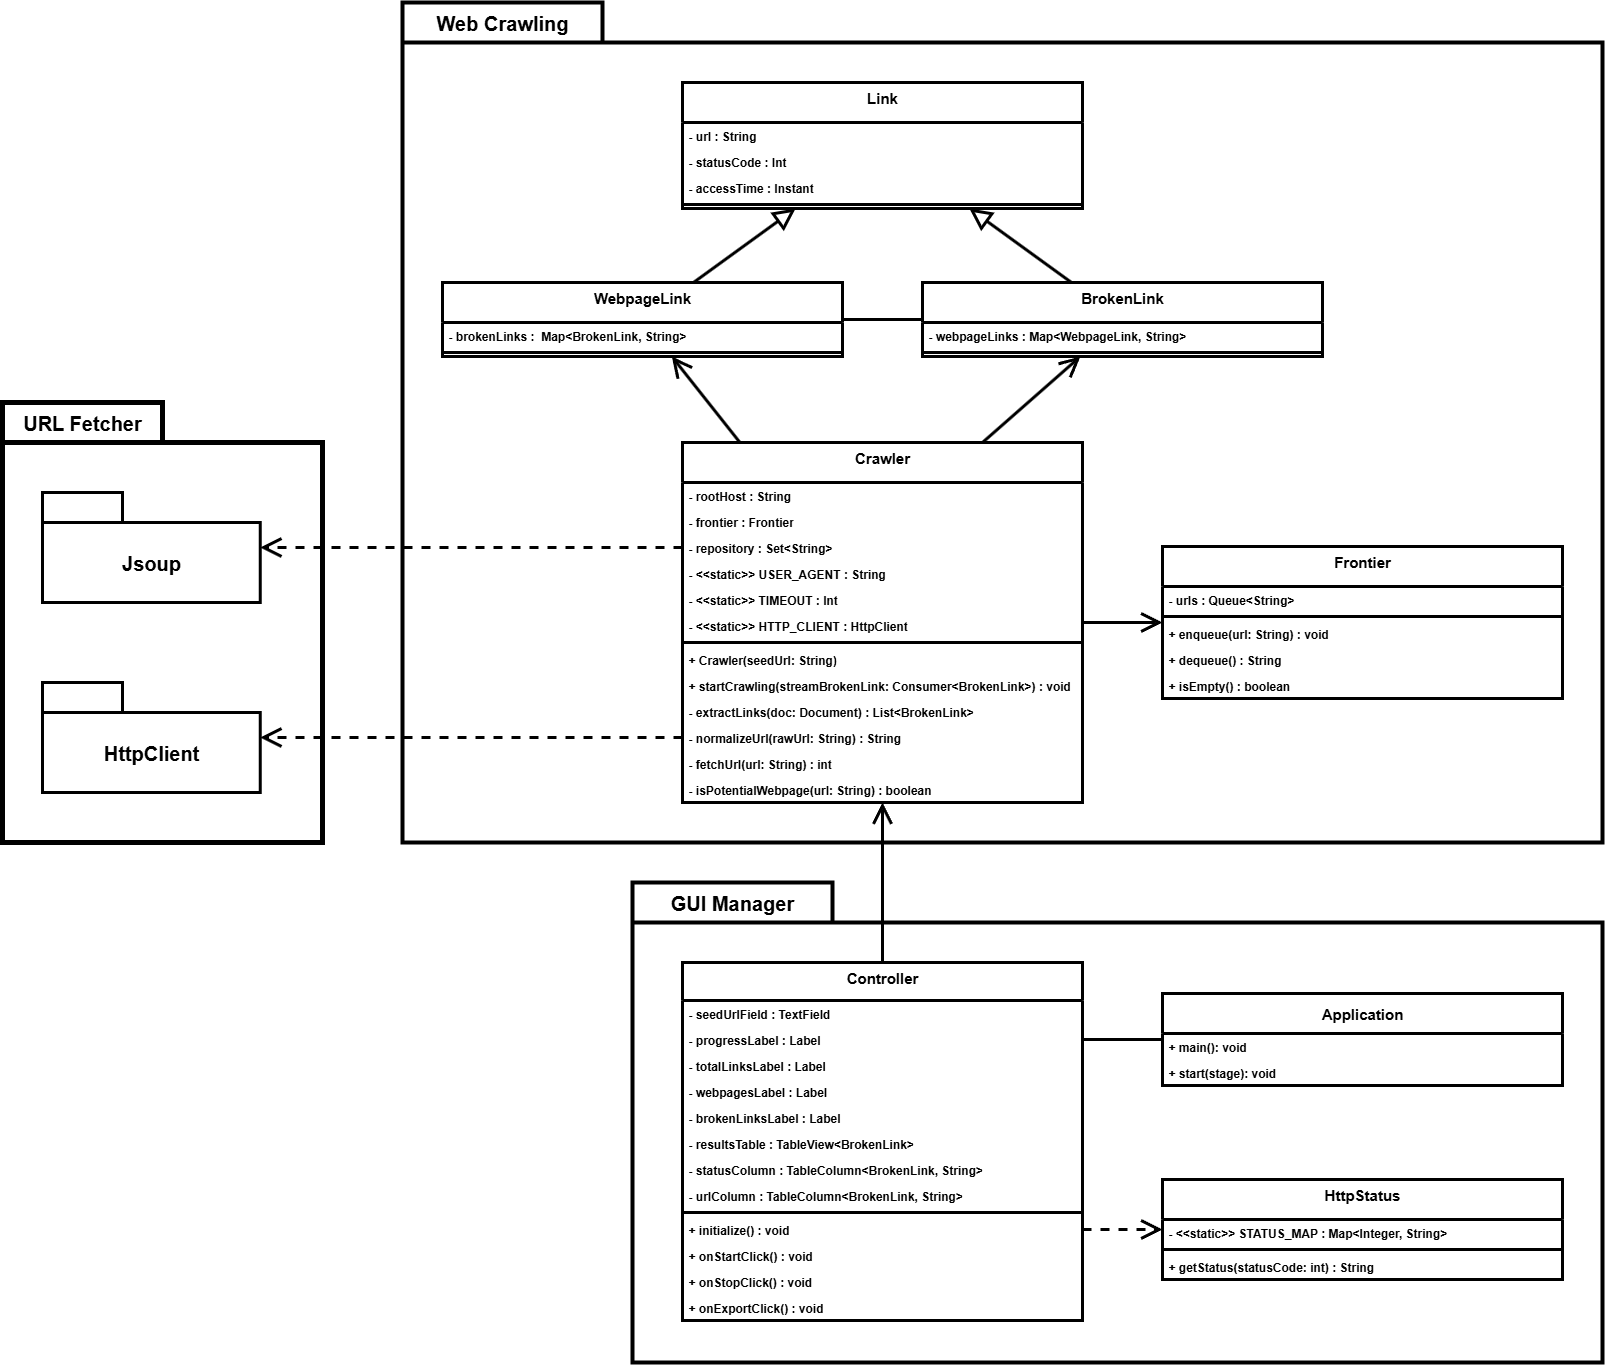
\includegraphics[width=0.95\textwidth]{Gambar/040100-class-diagram.png}
    \caption{Diagram kelas aplikasi}
    \label{fig:class-diagram}
\end{figure}

\begin{figure}[H]
    \centering
    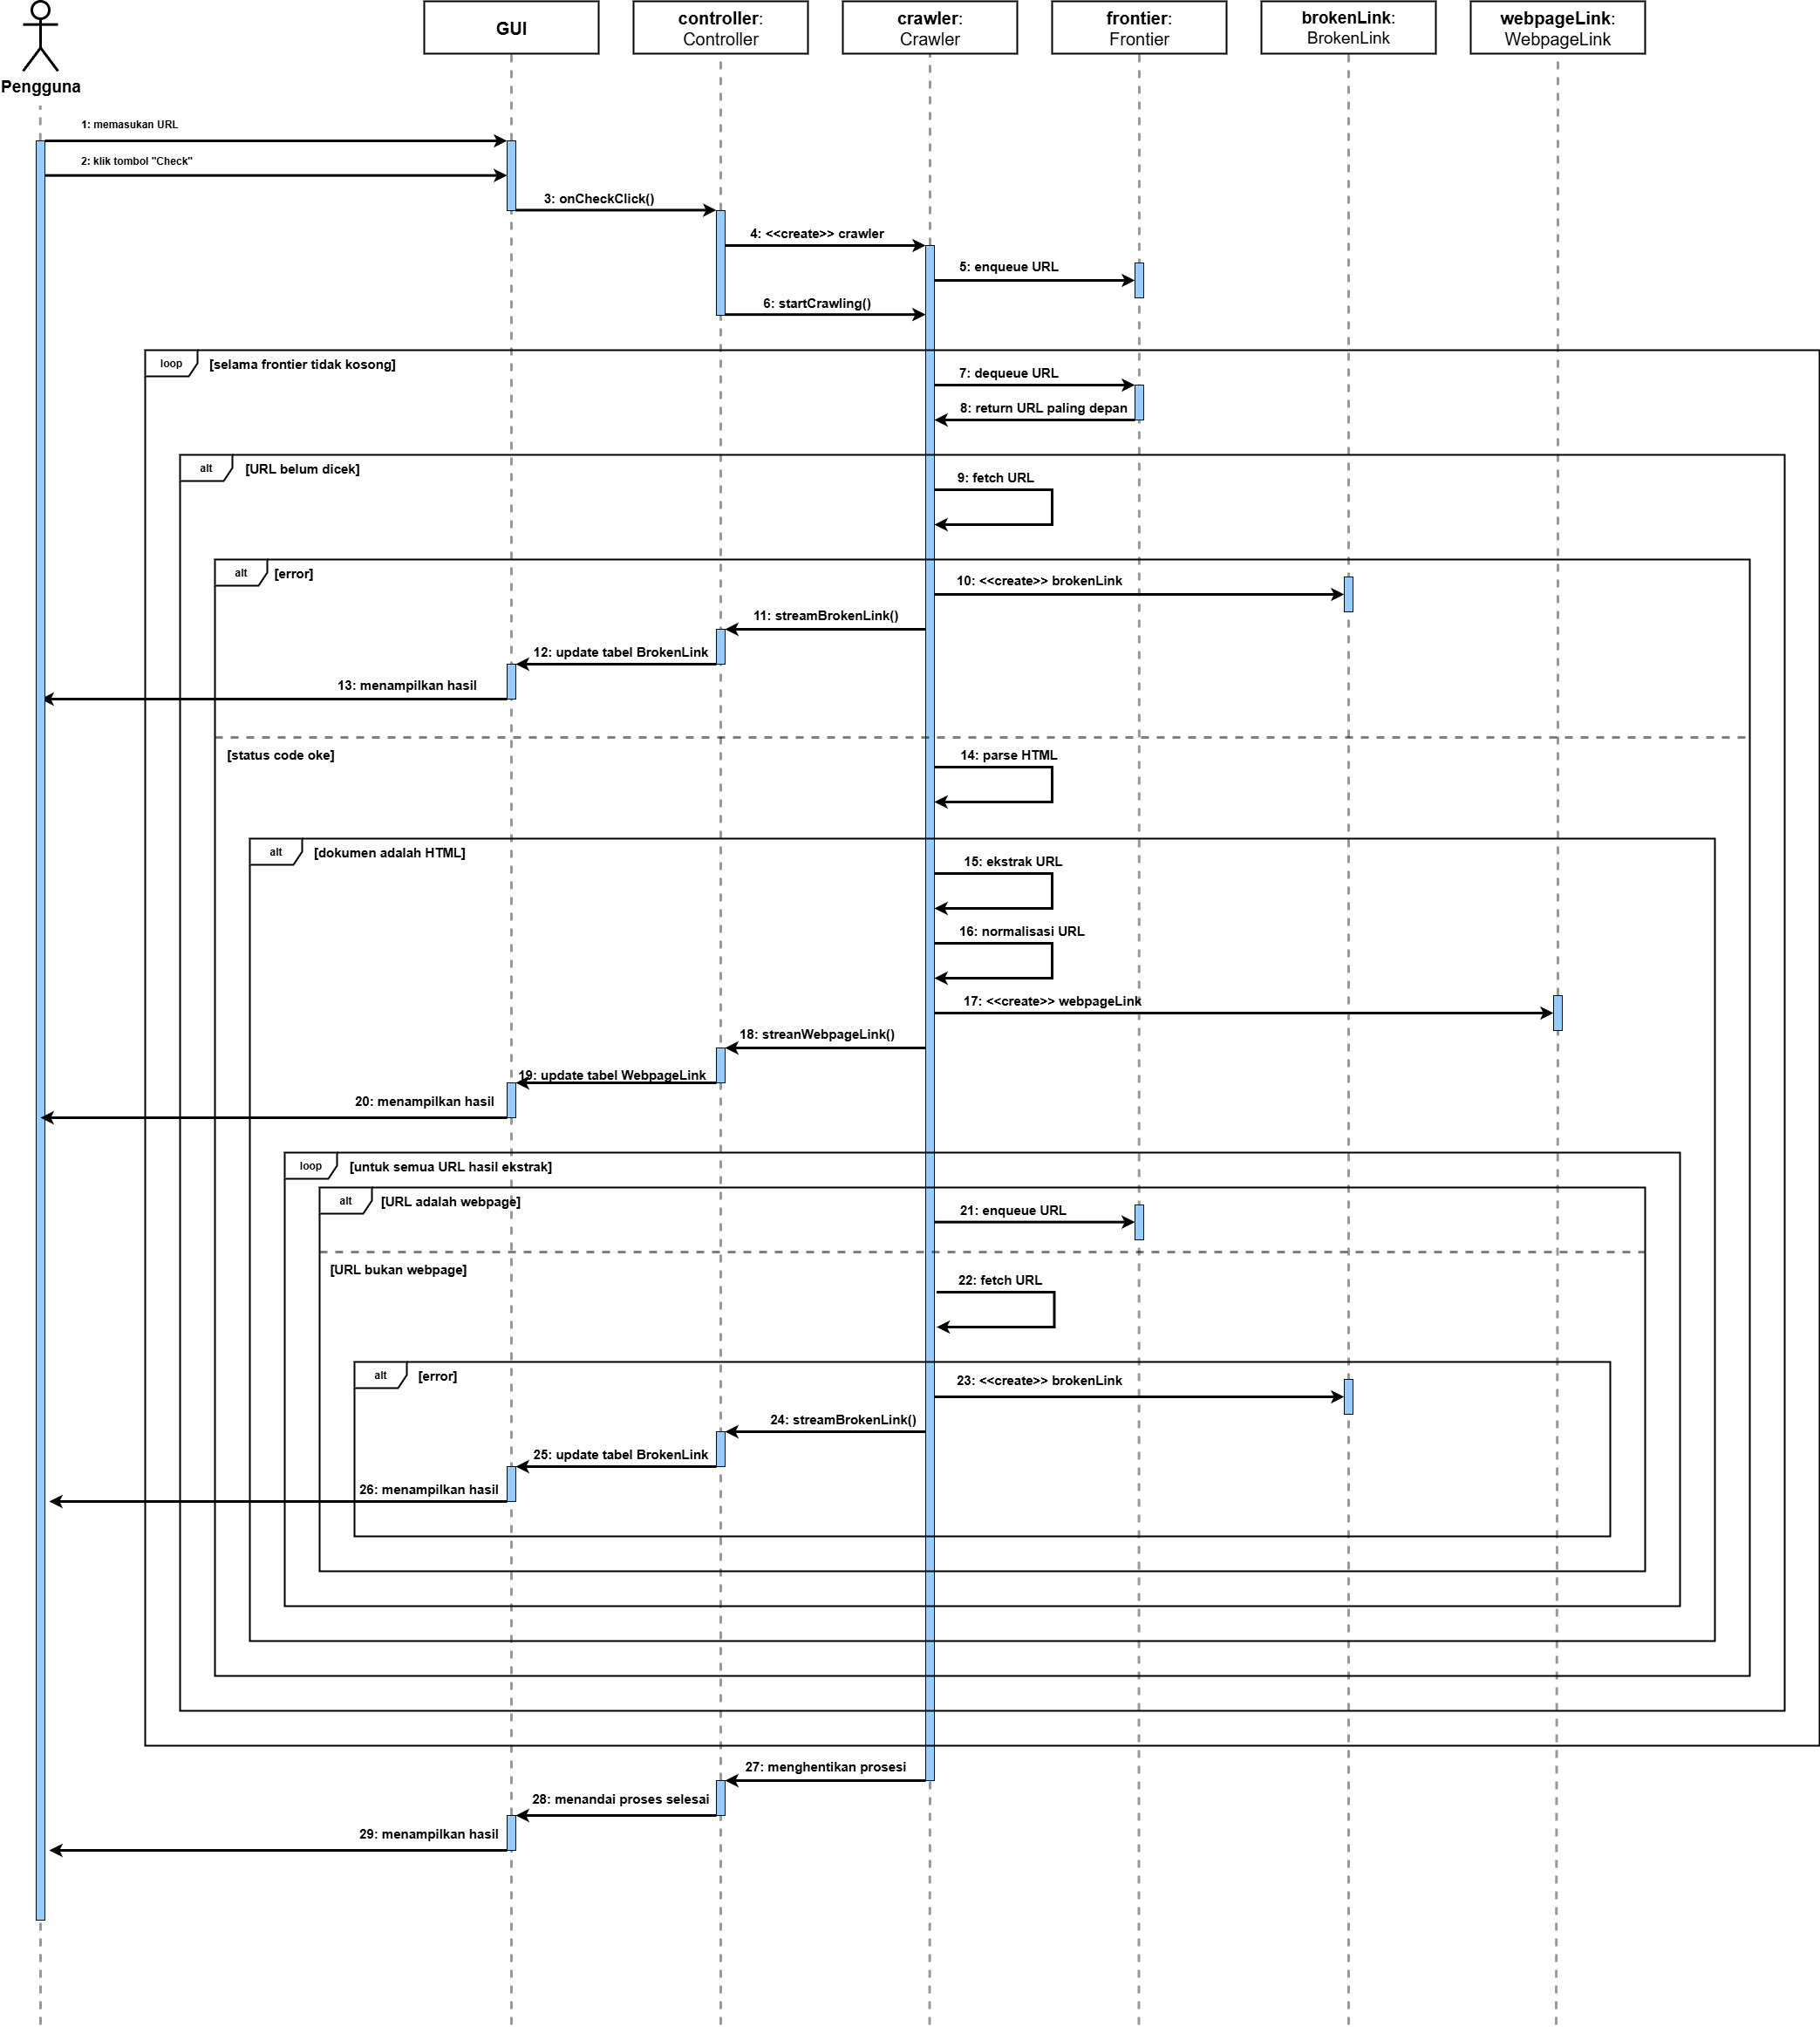
\includegraphics[width=1\textwidth]{Gambar/040200-sequence-diagram.png}
    \caption{Sequence diagram proses pemeriksaan tautan}
    \label{fig:sequence-crawl}
\end{figure}